Find the equation of line 
\begin{enumerate}[label=\thesection.\arabic*,ref=\thesection.\theenumi]
	\item passing through the point $\vec{P}(– 4, 3)$ with slope $\frac{1}{2}$.
\label{chapters/11/10/2/2}
\\
\solution
Since the normal vector 
\begin{align}
\vec{n}=\myvec{\frac{1}{2}\\ -1}\\
\end{align}
the desired equation \eqref{eq:geo-normal} is 
\begin{align}
\vec{n}^\top \brak{\vec{x}-\vec{P}}&= 0 \\
\implies \myvec{\frac{1}{2}&-1}{\vec{x}}&=-5
\end{align}
See 
		\figref{fig:chapters/11/10/2/2/Figure}.
\begin{figure}[h]
\centering
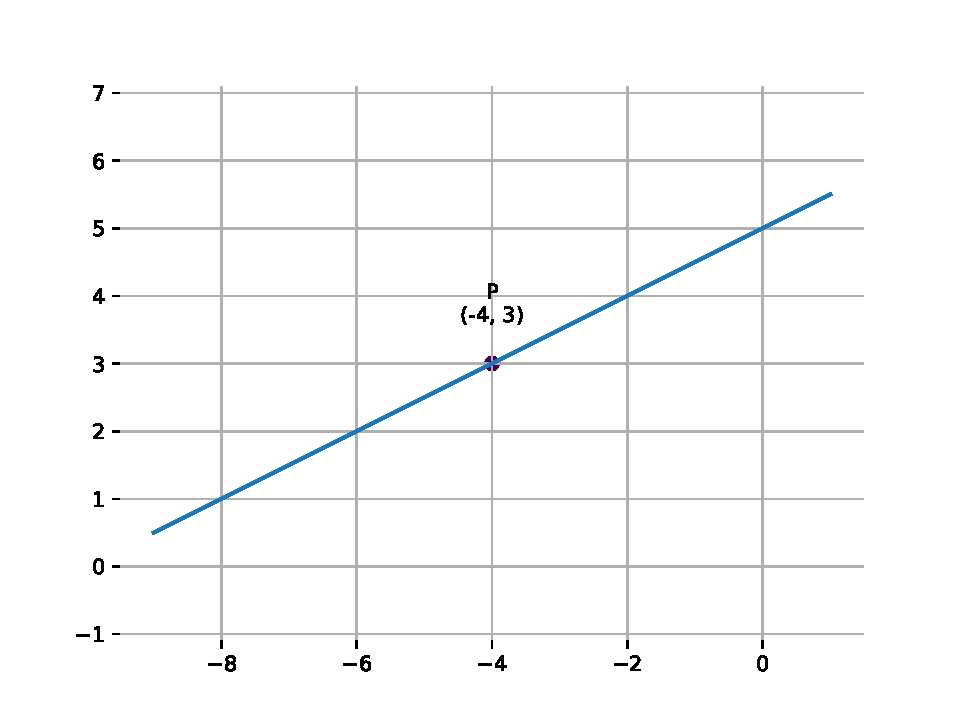
\includegraphics[width=\columnwidth]{chapters/11/10/2/2/figs/fig.pdf}
\caption{}
		\label{fig:chapters/11/10/2/2/Figure}
\end{figure}

	\item passing through $\myvec{0\\0}$ with slope $m$.\\
\label{chapters/11/10/2/3}
\solution
\iffalse
\documentclass[12pt]{article}
\usepackage{graphicx}
%\documentclass[journal,12pt,twocolumn]{IEEEtran}
\usepackage[none]{hyphenat}
\usepackage{graphicx}
\usepackage{listings}
\usepackage[english]{babel}
\usepackage{graphicx}
\usepackage{caption}
\usepackage[parfill]{parskip}
\usepackage{hyperref}
\usepackage{booktabs}
%\usepackage{setspace}\doublespacing\pagestyle{plain}
\def\inputGnumericTable{}
\usepackage{color}                                            %%
    \usepackage{array}                                            %%
    \usepackage{longtable}                                        %%
    \usepackage{calc}                                             %%
    \usepackage{multirow}                                         %%
    \usepackage{hhline}                                           %%
    \usepackage{ifthen}
\usepackage{array}
\usepackage{amsmath}   % for having text in math mode
\usepackage{parallel,enumitem}
\usepackage{listings}
\lstset{
language=tex,
frame=single, 
breaklines=true
}
  
%Following 2 lines were added to remove the blank page at the beginning
\usepackage{atbegshi}% http://ctan.org/pkg/atbegshi
\AtBeginDocument{\AtBeginShipoutNext{\AtBeginShipoutDiscard}}
%
%New macro definitions
\newcommand{\mydet}[1]{\ensuremath{\begin{vmatrix}#1\end{vmatrix}}}
\providecommand{\brak}[1]{\ensuremath{\left(#1\right)}}
\providecommand{\norm}[1]{\left\lVert#1\right\rVert}
\newcommand{\solution}{\noindent \textbf{Solution: }}
\newcommand{\myvec}[1]{\ensuremath{\begin{pmatrix}#1\end{pmatrix}}}
\let\vec\mathbf
\begin{document}
\begin{center}
\title{\textbf{Straight Lines}}
\date{\vspace{-5ex}} %Not to print date automatically
\maketitle
\end{center}
\setcounter{page}{1}
\section*{11$^{th}$ Maths - Chapter 10}
This is Problem-3 from Exercise 10.2
\begin{enumerate}
		\fi
		Line passing through point $\vec{A}=\myvec{0\\0}$ is given by,
\begin{align}
	\vec{n}^\top \brak{\vec{x}-\vec{A}} &= 0\label{eq:11/10/2/31}
\end{align}
Where,
		\begin{align}
			\vec{n} =\myvec{m \\ -1}
		\end{align}
		Substituting $\vec{A}$ and $\vec{n}$ in equation \eqref{eq:11/10/2/31}
		\begin{align}
			\myvec{m & -1}\brak{\vec{x}-\myvec{0\\0}} &=0\\
\implies			\myvec{m & -1}\vec{x} &= 0
		\end{align}
Line segment passing through $\myvec{0\\0}$ with slope $m = 2$ is shown in Fig. \ref{fig:11/10/2/3Fig1}
\begin{figure}[!h]
\begin{center}
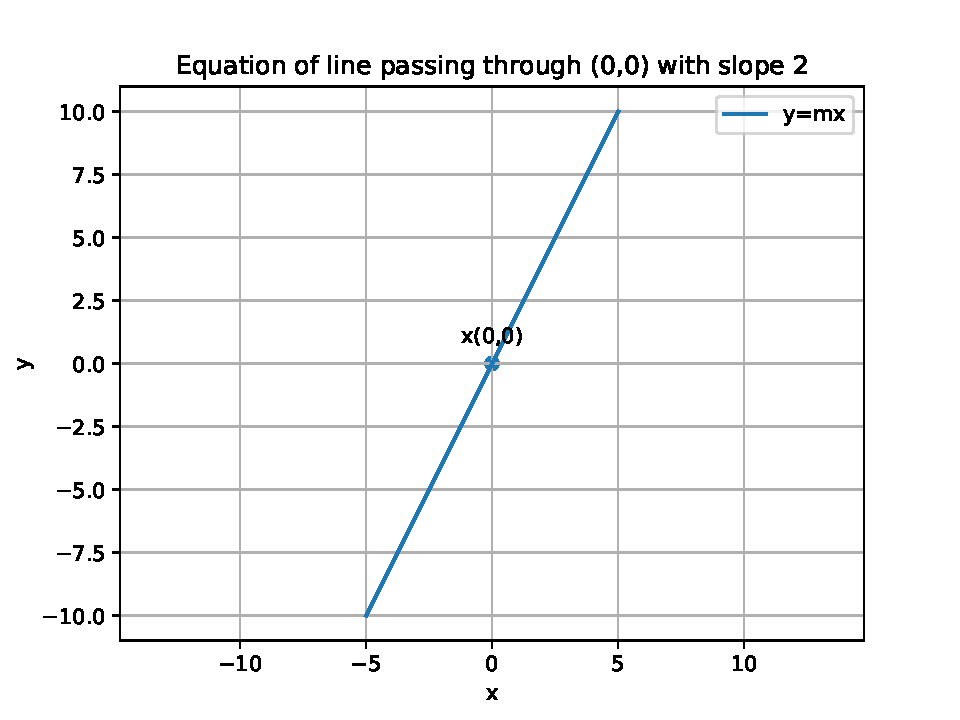
\includegraphics[width=\columnwidth]{chapters/11/10/2/3/figs/fig.pdf}
\end{center}
\caption{}
\label{fig:11/10/2/3Fig1}
\end{figure}

    \item passing through 
    $\vec{A} = \myvec{2\\2\sqrt{3}}$ and inclined with the x-axis at an angle 
    of 75\textdegree.
\label{chapters/11/10/2/4}
\\
    \solution 
    \begin{align}
	    \vec{n} &= \myvec{-1\\2+\sqrt{3}}
        \label{eq:11/10/2/4normal-vec}
	\\
	    \implies
        \implies \vec{n}^\top\vec{x} = \vec{n}^\top\vec{A} &= 4\brak{\sqrt{3}+1} \\
        \implies \myvec{-1&2+\sqrt{3}}\vec{x} &=\myvec{-1&2+\sqrt{3}}\myvec{2\\2\sqrt{3}}  
	    \\
	    &= 4\brak{\sqrt{3}+1}
        \label{eq:11/10/2/4line}
    \end{align}
is the desired equation.  See \figref{fig:11/10/2/4line}.
    \begin{figure}[!ht]
        \centering
        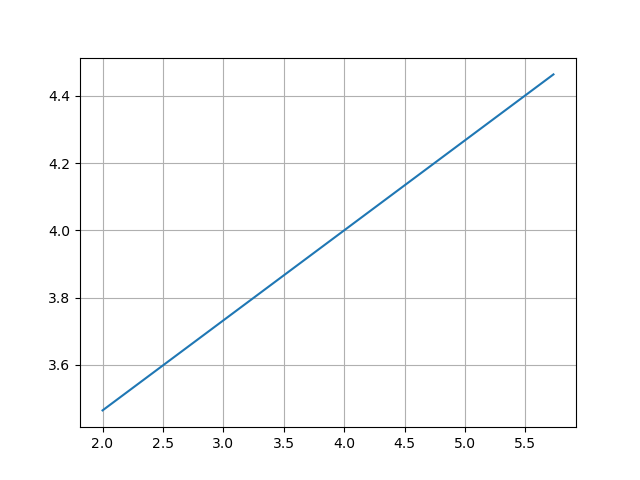
\includegraphics[width=\columnwidth]{chapters/11/10/2/4/figs/line.png}
        \caption{}
        \label{fig:11/10/2/4line}
    \end{figure}

\item intersecting the x-axis at a distance of 3 units to the left of origin with slope of -2.
\label{chapters/11/10/2/5}
\\
\solution 
		From the given information,
\begin{align}		
	\vec{A}=\myvec{-3\\0},\,
\vec{n} = \myvec{2 \\1}.
\end{align}
The desired equation of the line is
\begin{align}
\implies	\myvec { 2 & 1 } \brak{ \vec{x} - \myvec{ -3 \\ 0}} &= 0  \\
	\text{or, }	\myvec{ 2 & 1} \vec{x}  &= -6
        \label{eq:chapters/11/10/2/5/1}
\end{align}
See \figref{fig:chapters/11/10/2/5/Fig1}.
\begin{figure}[H]
	\begin{center}
		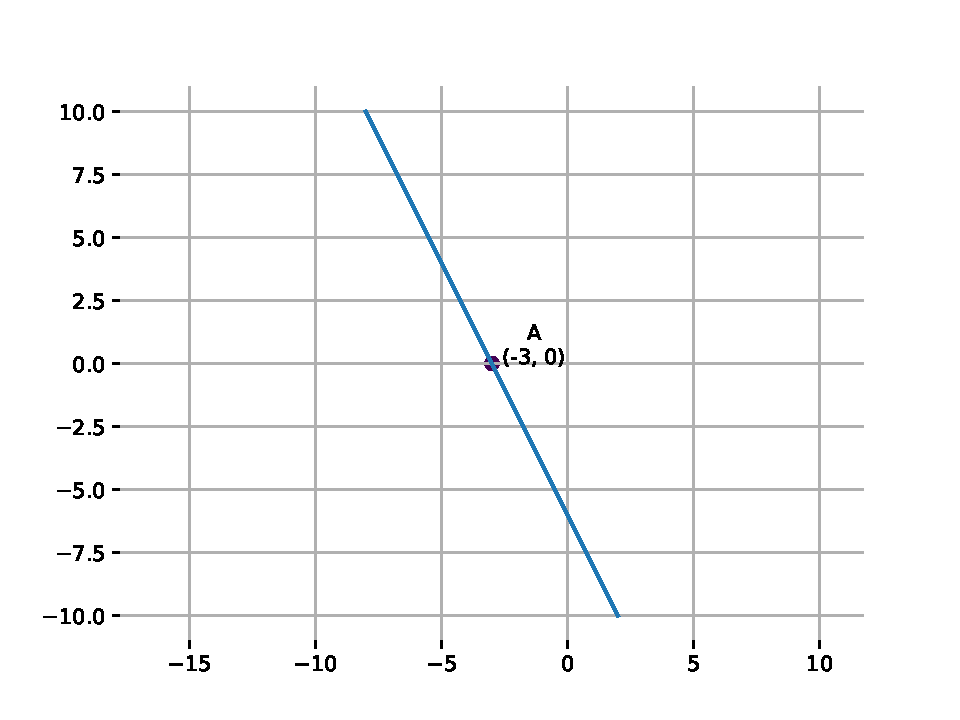
\includegraphics[width=0.75\columnwidth]{chapters/11/10/2/5/figs/fig.pdf}
	\end{center}
\caption{}
\label{fig:chapters/11/10/2/5/Fig1}
\end{figure}


\item intersecting the y-axis at a distance of 2 units above the origin and making an
angle of $30\degree$ with positive direction of the x-axis.
\\
\solution 
\iffalse
\documentclass[journal,12pt,twocolumn]{IEEEtran}
\usepackage{setspace}
\usepackage{gensymb}
\usepackage{xcolor}
\usepackage{caption}
\singlespacing
\usepackage{siunitx}
\usepackage[cmex10]{amsmath}
\usepackage{mathtools}
\usepackage{hyperref}
\usepackage{amsthm}
\usepackage{mathrsfs}
\usepackage{txfonts}
\usepackage{stfloats}
\usepackage{cite}
\usepackage{cases}
\usepackage{subfig}
\usepackage{longtable}
\usepackage{multirow}
\usepackage{enumitem}
\usepackage{bm}
\usepackage{mathtools}
\usepackage{listings}
\usepackage{tikz}
\usetikzlibrary{shapes,arrows,positioning}
\usepackage{circuitikz}
\renewcommand{\vec}[1]{\boldsymbol{\mathbf{#1}}}
\DeclareMathOperator*{\Res}{Res}
\renewcommand\thesection{\arabic{section}}
\renewcommand\thesubsection{\thesection.\arabic{subsection}}
\renewcommand\thesubsubsection{\thesubsection.\arabic{subsubsection}}

\renewcommand\thesectiondis{\arabic{section}}
\renewcommand\thesubsectiondis{\thesectiondis.\arabic{subsection}}
\renewcommand\thesubsubsectiondis{\thesubsectiondis.\arabic{subsubsection}}
\hyphenation{op-tical net-works semi-conduc-tor}

\lstset{
language=Python,
frame=single, 
breaklines=true,
columns=fullflexible
}
\begin{document}
\theoremstyle{definition}
\newtheorem{theorem}{Theorem}[section]
\newtheorem{problem}{Problem}
\newtheorem{proposition}{Proposition}[section]
\newtheorem{lemma}{Lemma}[section]
\newtheorem{corollary}[theorem]{Corollary}
\newtheorem{example}{Example}[section]
\newtheorem{definition}{Definition}[section]
\newcommand{\BEQA}{\begin{eqnarray}}
        \newcommand{\EEQA}{\end{eqnarray}}
\newcommand{\define}{\stackrel{\triangle}{=}}
\newcommand{\myvec}[1]{\ensuremath{\begin{pmatrix}#1\end{pmatrix}}}
\newcommand{\mydet}[1]{\ensuremath{\begin{vmatrix}#1\end{vmatrix}}}
\bibliographystyle{IEEEtran}
\providecommand{\nCr}[2]{\,^{#1}C_{#2}} % nCr
\providecommand{\nPr}[2]{\,^{#1}P_{#2}} % nPr
\providecommand{\mbf}{\mathbf}
\providecommand{\pr}[1]{\ensuremath{\Pr\left(#1\right)}}
\providecommand{\qfunc}[1]{\ensuremath{Q\left(#1\right)}}
\providecommand{\sbrak}[1]{\ensuremath{{}\left[#1\right]}}
\providecommand{\lsbrak}[1]{\ensuremath{{}\left[#1\right.}}
\providecommand{\rsbrak}[1]{\ensuremath{{}\left.#1\right]}}
\providecommand{\brak}[1]{\ensuremath{\left(#1\right)}}
\providecommand{\lbrak}[1]{\ensuremath{\left(#1\right.}}
\providecommand{\rbrak}[1]{\ensuremath{\left.#1\right)}}
\providecommand{\cbrak}[1]{\ensuremath{\left\{#1\right\}}}
\providecommand{\lcbrak}[1]{\ensuremath{\left\{#1\right.}}
\providecommand{\rcbrak}[1]{\ensuremath{\left.#1\right\}}}
\theoremstyle{remark}
\newtheorem{rem}{Remark}
\newcommand{\sgn}{\mathop{\mathrm{sgn}}}
\newcommand{\rect}{\mathop{\mathrm{rect}}}
\newcommand{\sinc}{\mathop{\mathrm{sinc}}}
\providecommand{\abs}[1]{\left\vert#1\right\vert}
\providecommand{\res}[1]{\Res\displaylimits_{#1}}
\providecommand{\norm}[1]{\lVert#1\rVert}
\providecommand{\mtx}[1]{\mathbf{#1}}
\providecommand{\mean}[1]{E\left[ #1 \right]}
\providecommand{\fourier}{\overset{\mathcal{F}}{ \rightleftharpoons}}
\providecommand{\ztrans}{\overset{\mathcal{Z}}{ \rightleftharpoons}}
\providecommand{\system}[1]{\overset{\mathcal{#1}}{ \longleftrightarrow}}
\newcommand{\solution}{\noindent \textbf{Solution: }}
\providecommand{\dec}[2]{\ensuremath{\overset{#1}{\underset{#2}{\gtrless}}}}
\let\StandardTheFigure\thefigure
\def\putbox#1#2#3{\makebox[0in][l]{\makebox[#1][l]{}\raisebox{\baselineskip}[0in][0in]{\raisebox{#2}[0in][0in]{#3}}}}
\def\rightbox#1{\makebox[0in][r]{#1}}
\def\centbox#1{\makebox[0in]{#1}}
\def\topbox#1{\raisebox{-\baselineskip}[0in][0in]{#1}}
\def\midbox#1{\raisebox{-0.5\baselineskip}[0in][0in]{#1}}

\vspace{3cm}
\title{11.10.2.6}
\author{Lokesh Surana}
\maketitle
\section*{Class 11, Chapter 10, Exercise 2.6}


\solution 
\fi
The direction vector of the line is given by
\begin{align}
    \vec{m} = \myvec{1 \\ \tan(30\degree)} = \myvec{1 \\ \frac{1}{\sqrt{3}}}
\end{align}
The normal vector $\vec{n}$ to the line is given by
\begin{align}
    \vec{n} =  \myvec{-\frac{1}{\sqrt{3}} \\ 1}
\end{align}
The line is passing through the point 
\begin{align}
    \vec{A} = \myvec{0 \\ 2}
\end{align}
Hence, 
the equation of the line is given by
\begin{align}
    \vec{n}^\top\brak{\vec{x}-\vec{A}} &= 0 \\
    \implies \myvec{-\frac{1}{\sqrt{3}}&1}\brak{ \vec{x} - \myvec{0 \\ 2}} &= 0  \\
    \text{or, }	\myvec{-\frac{1}{\sqrt{3}}&1} \vec{x}  &= 2
\end{align}
%
\begin{figure}[!htb]
    \centering
    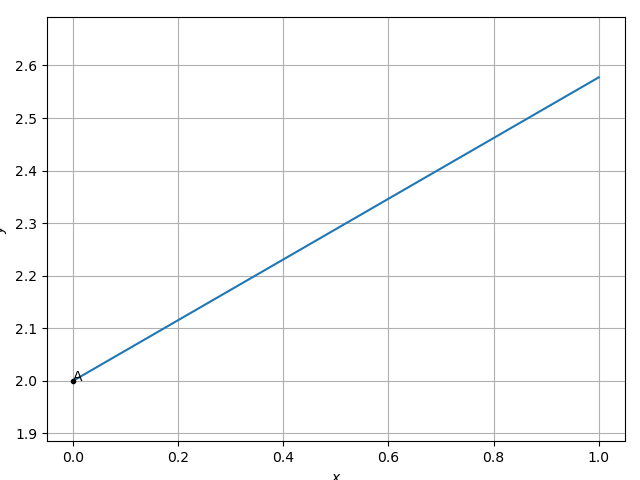
\includegraphics[width=\columnwidth]{chapters/11/10/2/6/figs/line.png}
    \caption{}
    \label{fig:chapters/11/10/2/6/line}
\end{figure}


\item Find the equation of the line passing through the points $\vec{A}\myvec{-1\\1}$ and $\vec{B}\myvec{2\\-4}$.
\\
\solution 
\begin{align}
	\vec{m} &= \vec{A} - \vec{B}
= \myvec{-3\\5}
\implies
\vec{n} &= \myvec{5\\3}
\end{align}
Thus, the equation of line is
\begin{align}
 \myvec{ 5 & 3}\vec{x}  &= -2
\end{align}
See 
   \figref{fig:chapters/11/10/2/7/Line_AB}.
\begin{figure}[h!]
  \centering
   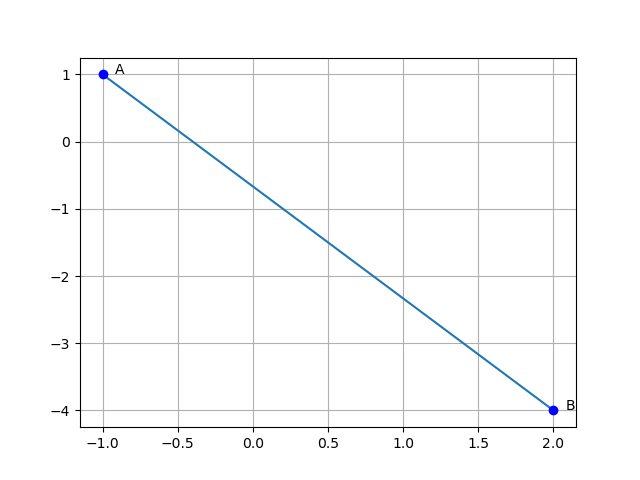
\includegraphics[width=\linewidth]{chapters/11/10/2/7/figs/Figure_1.png}
   \caption{}
   \label{fig:chapters/11/10/2/7/Line_AB}
\end{figure}





\item Find the equation of line whose perpendicular distance from the origin is 5 units and the angle made by the perpendicular with the positive $x$-axis is $30\degree$.
\label{chapters/11/10/2/8}
\\
\solution
			From 
\eqref{eq:chapters/11/10/2/8-final},
		Thus, the equation of lines are
\begin{align}
	\myvec{\frac{\sqrt{3}}{2}& \frac{1}{2}}\vec{x}=\pm5
\end{align}
See 
\figref{fig:chapters/11/10/2/8/Fig1}.
\begin{figure}[H]
\begin{center}
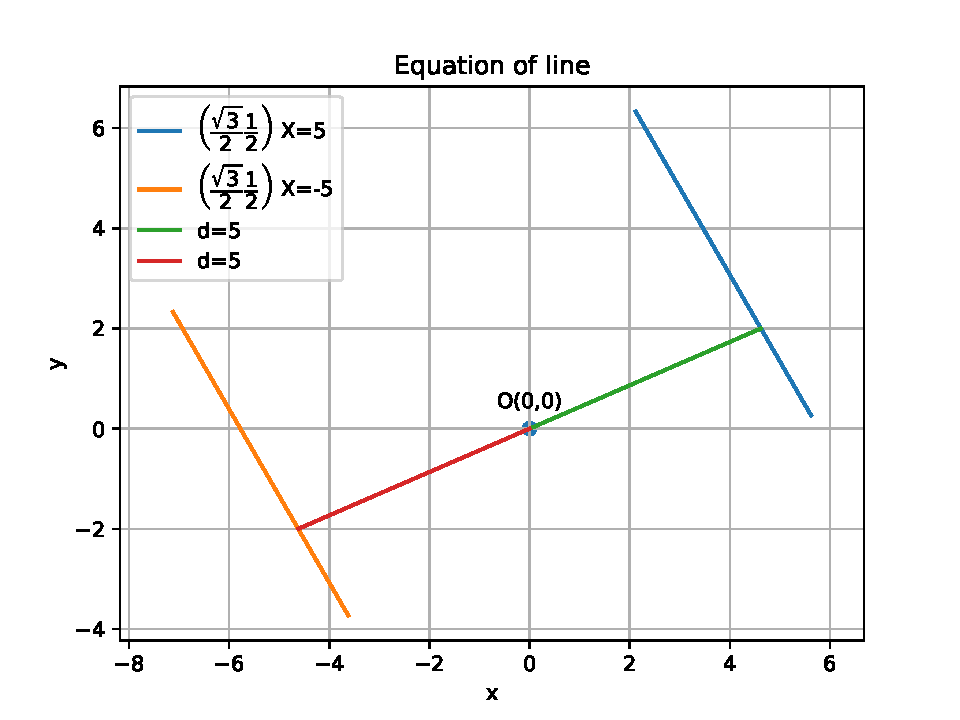
\includegraphics[width=0.75\columnwidth]{chapters/11/10/2/8/figs/fig.pdf}
\end{center}
\caption{}
\label{fig:chapters/11/10/2/8/Fig1}
\end{figure}

\item 
The vertices of triangle $PQR$ are $\vec{P}(2,1), \vec{Q}(-2,3), \vec{R}(4,5)$. Find the equation of the median through $\vec{R}$.
\label{chapters/11/10/2/9}
\\
\solution
	\begin{figure}[H]
		\centering
 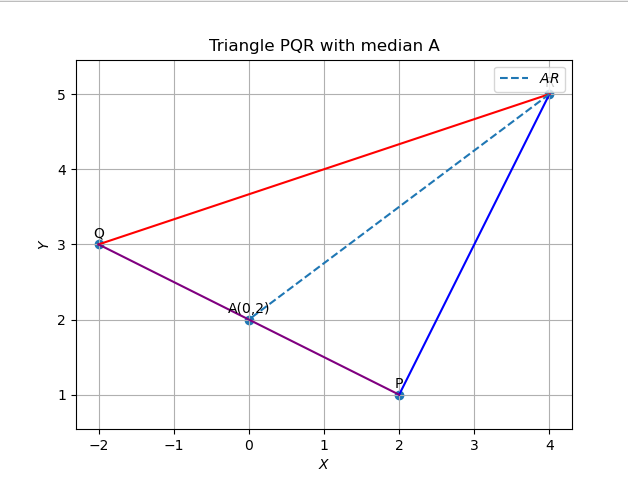
\includegraphics[width=0.75\columnwidth]{chapters/11/10/2/9/figs/line.png}
		\caption{}
		\label{fig:11/10/2/9}
  	\end{figure}
	See Fig. 
		\ref{fig:11/10/2/9}.
Using section formula, the mid point of $PQ$ is
\begin{align}
\vec{A} = \frac{\vec{P} +\vec{Q} }{2}
	= {\myvec{0\\2}}
\end{align} 
Following the approach in \probref{chapters/11/10/2/7},
\begin{align*}
	\augvec{2}{1}{ 
	4 & 5 & 1
	\\  
	0 & 2 & 1
	}
	\xleftrightarrow[R_2 \leftarrow 4R_2 ]{R_1 \leftarrow 2R_1 -5R_2}
	\augvec{2}{1}{ 
	8 & 0 & -3 
	\\ 
	0 & 8 & 4 
	}
	\implies \vec{n} = \frac{1}{8}\myvec{ -3 \\ 4}
\end{align*}
Thus,
the equation of the line is 
\begin{align}
	\myvec{-3 & 4}\vec{x} =8 
\end{align}

\item 
\label{chapters/11/10/2/10}
%	\begin{figure}[H]
		\centering
 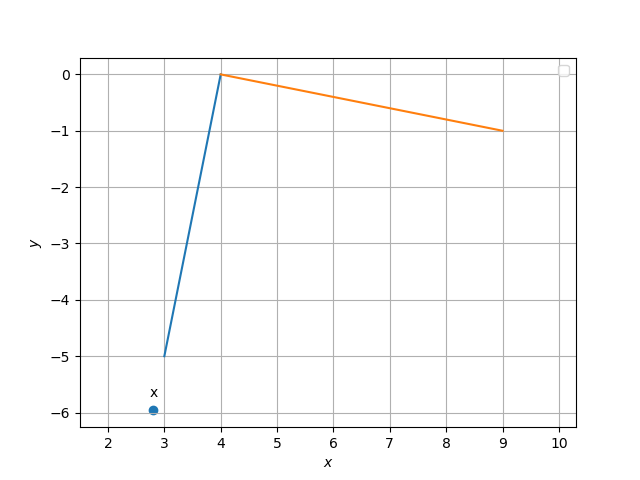
\includegraphics[width=0.75\columnwidth]{chapters/11/10/2/10/figs/Figure_1.png}
		\caption{}
		\label{fig:11/10/2/10}
  	\end{figure}
The normal vector is
\begin{align}
\vec{n} =\myvec{2 \\5} -  \myvec{-3 \\ 6} 
=\myvec{
    5\\
    -1
}
\end{align}
Thus, the equation of the line is 
\begin{align}
\myvec{
    5 &-1
	}\brak{\vec{x} - \myvec{-3 \\5}}
= 0
\\
\implies 
\myvec{
    5 &-1
	}\vec{x} 
= -20
\end{align}
See 
		\figref{fig:11/10/2/10}.

\item 
\label{chapters/11/10/2/11}
%\iffalse
\documentclass[journal,12pt,twocolumn]{article}
\usepackage{graphicx}
\graphicspath{{./figs/}}{}
\usepackage{amsmath,amssymb,amsfonts,amsthm}
\newcommand{\myvec}[1]{\ensuremath{\begin{pmatrix}#1\end{pmatrix}}}
\let\vec\mathbf
\title{
Matrix-Lines
}
\author{SHREYASH CHANDRA PUTTA}
\begin{document}
\maketitle
\tableofcontents

\section{Problem Statement}
\fi
A line perpendicular to the line segement joining the points (1,0) and (2,3) divides it in the ratio $1:n$. Find the equation of the line.
	\begin{figure}[!ht]
		\centering
 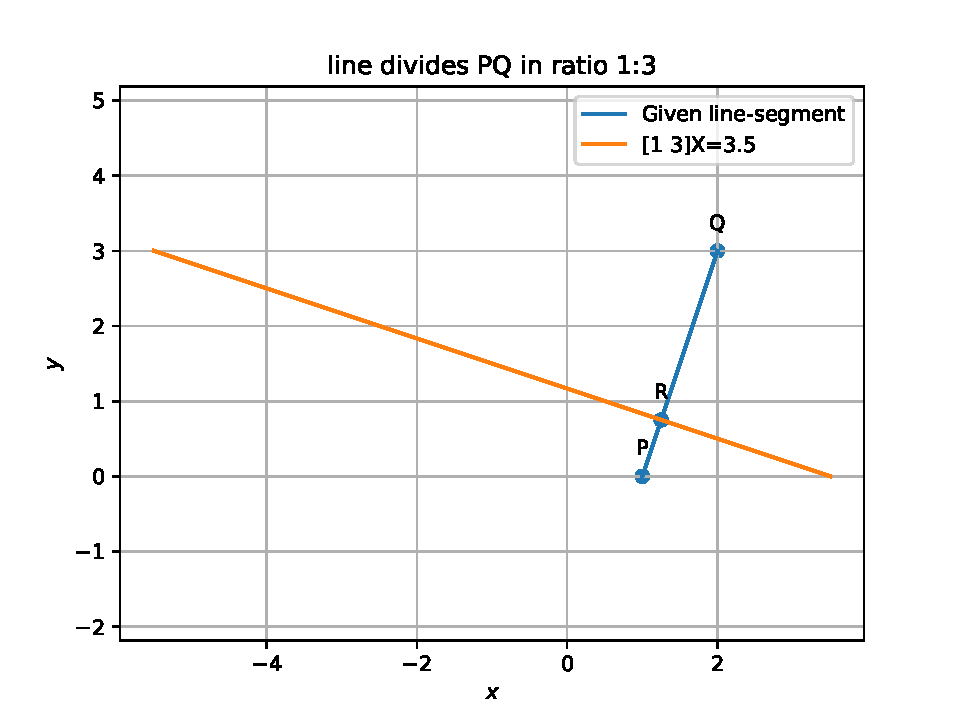
\includegraphics[width=\columnwidth]{chapters/11/10/2/11/figs/linefig.pdf}
		\caption{}
		\label{fig:11/10/2/11}
  	\end{figure}
	\\
	\solution 
\iffalse
(note: we are taking n as user Input) .

% 

\begin{table}[h]
    \centering
    \begin{tabular}{|c|c|c|}
       \hline
       \textbf{Symbol}&\textbf{Value}&\textbf{Description}  \\
       \hline
	    $\vec{P}$ & $\myvec{
		    1\\
		    0}$
	    & given point\\
        \hline
	    $\vec{Q}$ & $\myvec{2\\3}$
 & given point\\
        \hline
	    $\vec{R}$ & $\myvec{
  \frac{2+n}{1+n}\\
  \frac{3}{1+n}}$
 & intersecting point  \\
       \hline
    \end{tabular}
    \caption{Parameters}
    \label{tab:my_label}
\end{table}

%\section{Construction}

\begin{figure}[h]
    \centering
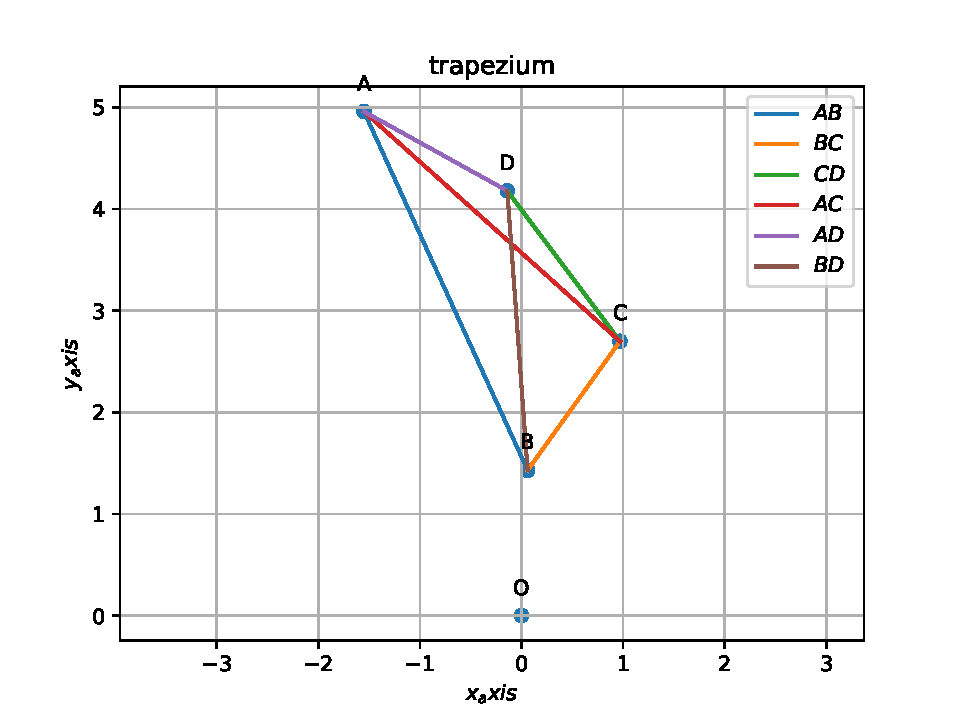
\includegraphics[width=\columnwidth]{fig/linefig.pdf}
    \caption{Equation of the required Straight Line}
    \label{fig:my_label}
\end{figure}




\section{Solution}

Given that resultant will divide the equation of line in the ratio 1:n and the line is perpendicular to line segment joining the points (1,0)and(2,3)  ) \\
%so, b = 9 - a  \\
\\
\fi 
Let 
\begin{align}
{\vec{P}}=\myvec{
  1\\
  0},
 {\vec{Q}}=\myvec{
  2\\
  3}
\end{align}
\iffalse
%	\vec{n^{\top}}
%	\myvec{
 % a\\
  %0}
  %= c \label{eq-1}
%\end{align}
\\
\fi
The direction vector of 
$PQ$ is 
\begin{align}
	\vec{m}=
     \vec{Q
 }-  \vec{P
 }
=
     \myvec{
  1\\
  3
 }
\end{align}
\iffalse
\\
We know, that position or  directional vector of points P and Q line segement used as the normal vector
\\
\\
 The general equation of the required perpendicular line is
 ${\vec{M^{\top}}\vec{X}} = c$.
 \\
 \\
 The perpendicular line cutting a line segment P and Q in ratio 1:n is passes through the point R.
 \fi
 Also, using section formula, 
 \begin{align}
	 \vec{R}=\frac{\vec{Q}+n\vec{P}}{1+n}
\end{align}
and the 
equation of line passing through ${\vec{R}}$ is
\begin{align}
	\vec{m}^{\top}\brak{\vec{x}-\vec{R}}=0
\\
\implies 
	   \myvec{
		   1 &  3}\vec{x}
	   &= \myvec{
  1\ 3}\myvec{
  \frac{2+n}{1+n}\\
  \frac{3}{1+n}} 
  \\
	&=	  \frac{11+n}{1+n} 
\end{align}
\iffalse



 
\section{Software}
Download the following code using,
\begin{table}[h]
    \centering
    \begin{tabular}{|c|}
    \hline \\
         svn co https://github.com/chanduputta/ \\FWC-Module1Assignments/blob/\\main/assignment4/line/lines3.py  \\
         \\
\hline
    \end{tabular}
\end{table}
\\
and execute the code by using command
\begin{center}
	\textbf{cmd:}
{Python3  lines3.py}\\
	\textbf{Then,}
{input your required n value}
\end{center}

\section{Conclusion}
\begin{center}
We found the equation of a line perpendicular to the line segement joining the points (1,0)and(2,3) divides it in the ratio 1:n .
\end{center}
\end{document}
\fi

\item 
\label{chapters/11/10/2/12}
%Let $(a,0)$  and  $(0,a)$ be the intercept points. 
\begin{align}
\vec{m} 
        &=   \myvec{
		a \\
		0 
		} - \myvec{
		   0 \\
		   a
		}  
        		  \equiv \myvec{
                           1 \\
			   -1 
		         } 
			 \\
			 \implies
\vec{n} &=  \myvec{
		     1 \\
		     1
	     } 
\end{align}
and 
the equation of the  line is
\begin{align}
	\myvec { 1 & 1 } \brak{ \vec{ x  - \myvec{ 2 \\
                                   3
			     }
		}}  &= 0  \\
\implies		\myvec{ 1 & 1} \vec{x}  &= 5 
        \label{eq:11/10/2/12/1}
\end{align}
See  \figref{fig:11/10/2/12/Fig1}.
\begin{figure}[H]
	\begin{center}
		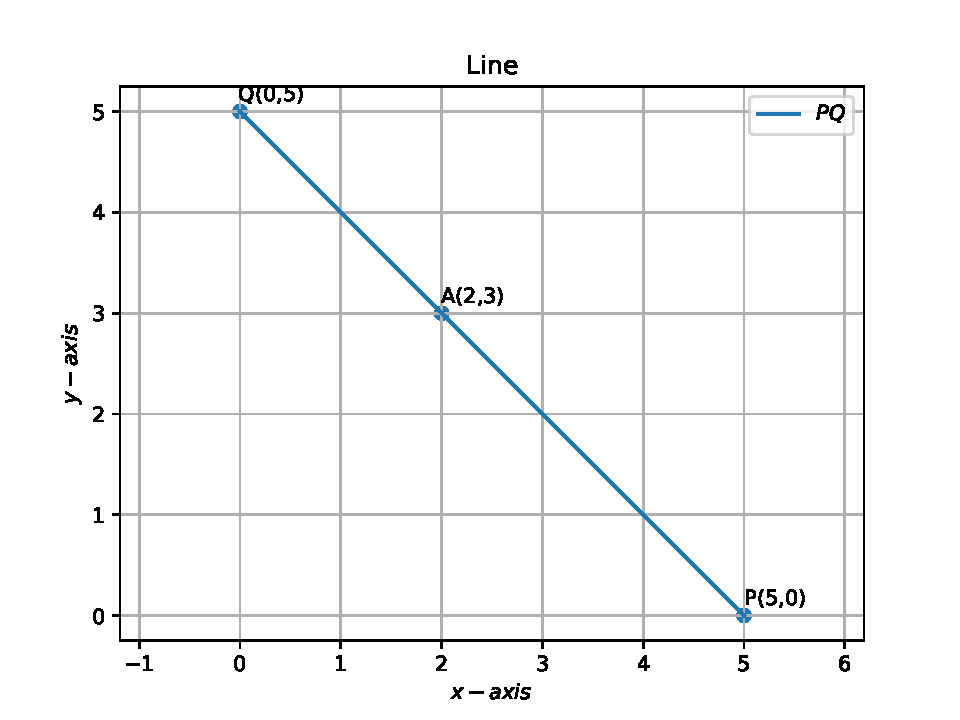
\includegraphics[width=0.75\columnwidth]{chapters/11/10/2/12/figs/problem12.pdf}
	\end{center}
\caption{}
\label{fig:11/10/2/12/Fig1}
\end{figure}


\item 
\label{chapters/11/10/2/13}
%Let  the intercept points be
\begin{align}
{\vec{P}}=\myvec{
  a\\
  0}
 , {\vec{Q}}=\myvec{
  0\\
  b}
  \text{ and }
   {\vec{R}}=\myvec{
  2\\
  2}
\end{align}
be the given point.  
Forming the collinearity matrix from 
		\eqref{prop:lin-dep-rank},
\begin{align}
	\myvec{ \vec{P}-\vec{Q} &\vec{P}-\vec{R}} 
	=
	 \myvec{
  a & a-2\\
  -b & -2
 }
\end{align}
which is singular if 
\begin{align}
 ab -2\brak{a+b} = 0
 \implies ab = 18
		\label{eq:11/10/2/13-a+b}
		\\
\because  a + b = 9.
\end{align}
$\therefore a,b$
are the roots of
\begin{align}
	x^2 -9x +18 = 0.
\end{align}
yielding
\begin{align}
	\myvec{a \\ b} = \myvec{6 \\ 3}, \myvec{3\\6}
\end{align}
Since 
\begin{align}
	\vec{m} = \myvec{a \\ -b},
	\vec{n} = \myvec{b \\ a} \equiv \myvec{1 \\ 2}, \myvec{2\\1}
\end{align}
Thus, the possible equations of the line are 
\begin{align}
\myvec{1 & 2}\vec{x} = 6
	\\
	\myvec{2&1}\vec{x} = 6
\end{align}
		See \figref{fig:11/10/2/13}.
	\begin{figure}[H]
		\centering
 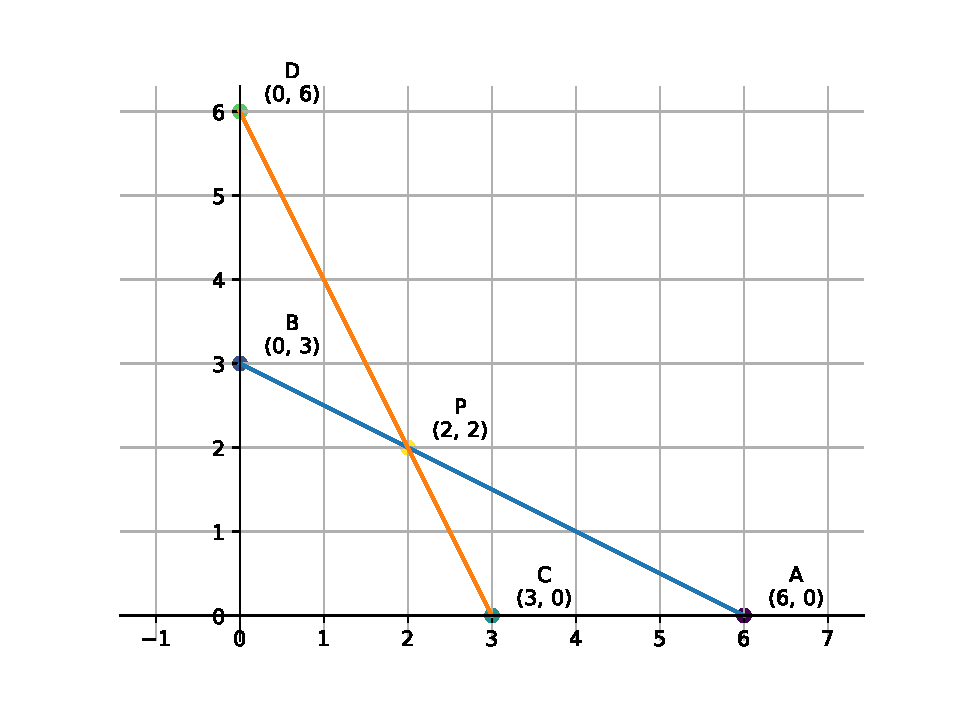
\includegraphics[width=0.75\columnwidth]{chapters/11/10/2/13/figs/fig.pdf}
		\caption{}
		\label{fig:11/10/2/13}
  	\end{figure}

\item 
\label{chapters/11/10/2/14}
%The equation of the first line is 
\begin{align}
	\myvec{\sqrt{3} &1}\myvec{\vec{x}-\myvec{0\\2}}&=0
	\\
	\implies 
	\myvec{\sqrt{3}&1}
	\vec{x}&=2
\end{align}
The equation of the second line is 
\begin{align}
	\myvec{\sqrt{3} &1}\myvec{\vec{x}-\myvec{0\\-2}}&=0
	\\
	\implies 
	\myvec{\sqrt{3}&1}
\vec{x}=-2
\end{align}
See
		\figref{fig:11/10/2/14}.
	\begin{figure}[!ht]
		\centering
 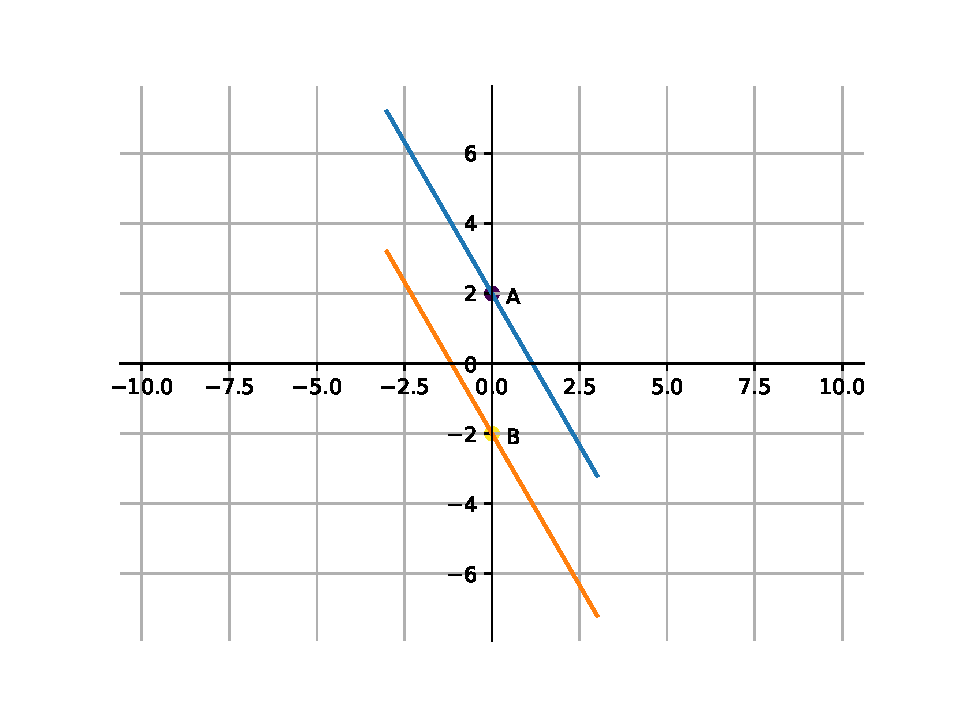
\includegraphics[width=\columnwidth]{chapters/11/10/2/14/figs/fig.pdf}
		\caption{}
		\label{fig:11/10/2/14}
  	\end{figure}

\item 
\label{chapters/11/10/2/15}
%It is obvious that the normal vector to the line is 
\begin{align}
\vec{n} =\myvec{2 \\ -9} -\vec{0} 
=\myvec{2 \\ -9}
\end{align}
Hence, the equation of the line is 
\begin{align}
	\myvec{2 & -9}\brak{\vec{x} - \myvec{2 \\ -9}}&= 0
	\\
	\implies 
	\myvec{2 & -9}\vec{x} &= 85
\end{align}
See 
		\figref{fig:11/10/2/15}.
	\begin{figure}[!ht]
		\centering
 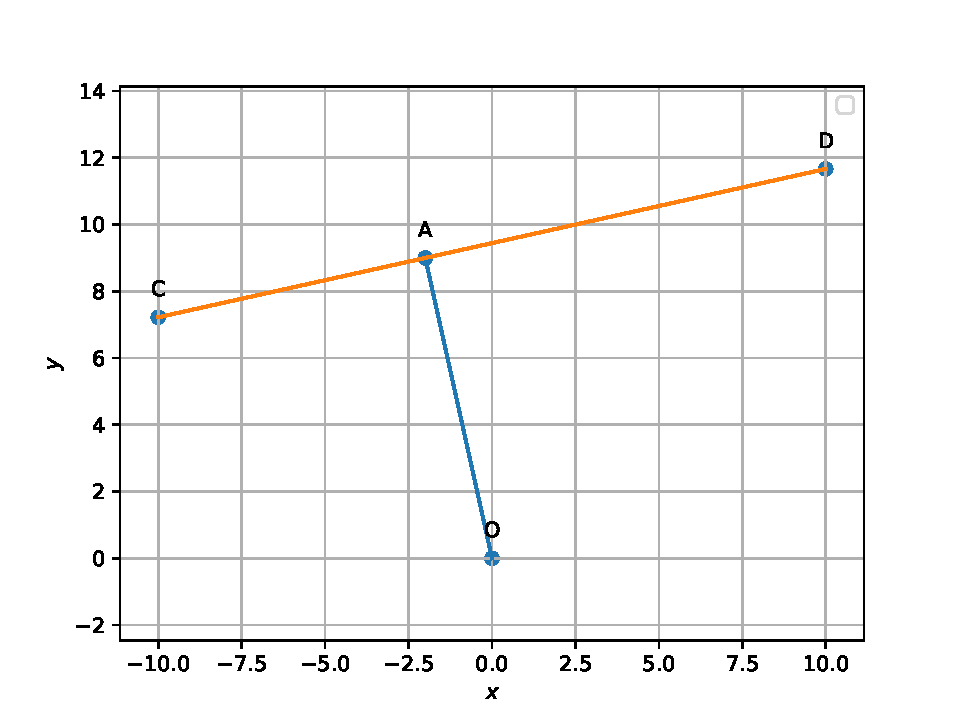
\includegraphics[width=\columnwidth]{chapters/11/10/2/15/figs/line.pdf}
		\caption{}
		\label{fig:11/10/2/15}
  	\end{figure}

\item 
$P(a,b)$ is the mid-point of the line segment between axes. Show that the equation of the line is $\frac{x}{a}+\frac{y}{b}=2$
\label{chapters/11/10/2/18}
\\
\solution
%\iffalse

\documentclass[12pt]{article}
\usepackage{graphicx}
\usepackage{amsmath}
\usepackage{mathtools}
\usepackage{gensymb}
\usepackage{amssymb}

\newcommand{\mydet}[1]{\ensuremath{\begin{vmatrix}#1\end{vmatrix}}}
\providecommand{\brak}[1]{\ensuremath{\left(#1\right)}}
\providecommand{\norm}[1]{\left\lVert#1\right\rVert}
\newcommand{\solution}{\noindent \textbf{Solution: }}
\newcommand{\myvec}[1]{\ensuremath{\begin{pmatrix}#1\end{pmatrix}}}
\let\vec\mathbf

\begin{document}
\begin{center}
\textbf\large{CLASS 11 CHAPTER-11 \\ LINES}

\end{center}
\section*{Excercise 10.2}


\solution
\fi
Let
\begin{align}
	\vec{A}&=x\vec{e_{1}},
	\vec{B}&=y\vec{e_{2}},
	\vec{P}&=\myvec{a\\b}
\end{align}
where
\begin{align}
	\vec{e_{1}}=\myvec{1\\0} \text{ and } \vec{e_{2}}=\myvec{0\\1}
\end{align}
as shown in Fig. \ref{fig:11/10/2/18Fig1}
\begin{figure}[!h]
	\begin{center} 
	    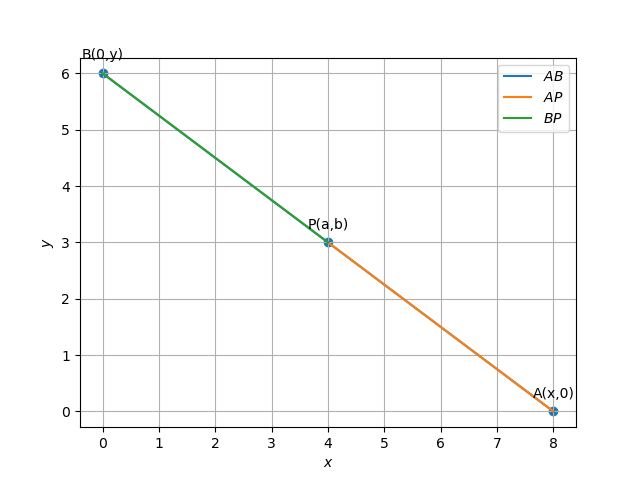
\includegraphics[width=\columnwidth]{chapters/11/10/2/18/figs/line1}
	\end{center}
\caption{}
\label{fig:11/10/2/18Fig1}
\end{figure}
Given that
\begin{align}
	\vec{P}&=\frac{\vec{A}+\vec{B}}{2}=\frac{x\vec{e_{1}}+y\vec{e_{2}}}{2}\\
\implies 	2\vec{P}&=x\vec{e_{1}}+y\vec{e_{2}}\\
	\vec{e_{1}}^{\top}\brak{2\vec{P}}&=\vec{e_{1}^{\top}}\brak{x\vec{e_{1}}+y\vec{e_{2}}}
=x\\				 
	\text{ and }\vec{e_{2}}^{\top}\brak{2\vec{P}}&=\vec{e_{2}^{\top}}\brak{x\vec{e_{1}}+y\vec{e_{2}}}
=y				 
\end{align}
Thus,
\begin{align}
	x&=2\vec{e_{1}}^{\top}\vec{P}=2a\\
	y&=2\vec{e_{2}}^{\top}\vec{P}=2b
\end{align}
yielding
\begin{align}
	\vec{A} &= 2a\vec{e_{1}}
	\vec{B} &= 2b\vec{e_{1}}
\end{align}
Thus, the direction vector of the line is 
\begin{align}
	\vec{m} &= \vec{A}-\vec{B}\\
	&=\myvec{a \\ -b}
\end{align}
and the normal vector is
\begin{align}
	\vec{n} = \myvec{b \\ a}
\end{align}
The equation of line passing through $\vec{P}$ is then obtained as
\begin{align}
	\vec{n}^{\top} \brak{\vec{x}-\vec{P}} &= 0\\
	\myvec{b & a}\vec{x} &= 2ab.
\end{align}



\item Point $\vec{R}\brak{h, k}$ divides a line segment between the axes in the ratio 1: 2. Find the equation of the line.
\label{chapters/11/10/2/19}
%\iffalse
\documentclass[journal,12pt,twocolumn]{IEEEtran}
\usepackage{setspace}
\usepackage{gensymb}
\singlespacing
\usepackage[cmex10]{amsmath}
\usepackage{amsthm}
\usepackage{mathrsfs}
\usepackage{txfonts}
\usepackage{stfloats}
\usepackage{bm}
\usepackage{cite}
\usepackage{cases}
\usepackage{subfig}
\usepackage{longtable}
\usepackage{multirow}
\usepackage{enumitem}
\usepackage{mathtools}
\usepackage{steinmetz}
\usepackage{tikz}
\usepackage{circuitikz}
\usepackage{verbatim}
\usepackage{tfrupee}
\usepackage[breaklinks=true]{hyperref}
\usepackage{tkz-euclide}
\usetikzlibrary{calc,math}
\usepackage{listings}
    \usepackage{color}                                            %%
    \usepackage{array}                                            %%
    \usepackage{longtable}                                        %%
    \usepackage{calc}                                             %%
    \usepackage{multirow}                                         %%
    \usepackage{hhline}                                           %%
    \usepackage{ifthen}                                           %%
  %optionally (for landscape tables embedded in another document): %%
    \usepackage{lscape}     
\usepackage{multicol}
\usepackage{chngcntr}
\DeclareMathOperator*{\Res}{Res}
\renewcommand\thesection{\arabic{section}}
\renewcommand\thesubsection{\thesection.\arabic{subsection}}
\renewcommand\thesubsubsection{\thesubsection.\arabic{subsubsection}}

\renewcommand\thesectiondis{\arabic{section}}
\renewcommand\thesubsectiondis{\thesectiondis.\arabic{subsection}}
\renewcommand\thesubsubsectiondis{\thesubsectiondis.\arabic{subsubsection}}

% correct bad hyphenation here
\hyphenation{op-tical net-works semi-conduc-tor}
\def\inputGnumericTable{}                                 %%

\lstset{
frame=single, 
breaklines=true,
columns=fullflexible
}

\begin{document}


\newtheorem{theorem}{Theorem}[section]
\newtheorem{problem}{Problem}
\newtheorem{proposition}{Proposition}[section]
\newtheorem{lemma}{Lemma}[section]
\newtheorem{corollary}[theorem]{Corollary}
\newtheorem{example}{Example}[section]
\newtheorem{definition}[problem]{Definition}
\newcommand{\BEQA}{\begin{eqnarray}}
\newcommand{\EEQA}{\end{eqnarray}}
\newcommand{\define}{\stackrel{\triangle}{=}}

\bibliographystyle{IEEEtran}
\providecommand{\mbf}{\mathbf}
\providecommand{\pr}[1]{\ensuremath{\Pr\left(#1\right)}}
\providecommand{\qfunc}[1]{\ensuremath{Q\left(#1\right)}}
\providecommand{\sbrak}[1]{\ensuremath{{}\left[#1\right]}}
\providecommand{\lsbrak}[1]{\ensuremath{{}\left[#1\right.}}
\providecommand{\rsbrak}[1]{\ensuremath{{}\left.#1\right]}}
\providecommand{\brak}[1]{\ensuremath{\left(#1\right)}}
\providecommand{\lbrak}[1]{\ensuremath{\left(#1\right.}}
\providecommand{\rbrak}[1]{\ensuremath{\left.#1\right)}}
\providecommand{\cbrak}[1]{\ensuremath{\left\{#1\right\}}}
\providecommand{\lcbrak}[1]{\ensuremath{\left\{#1\right.}}
\providecommand{\rcbrak}[1]{\ensuremath{\left.#1\right\}}}
\theoremstyle{remark}
\newtheorem{rem}{Remark}
\newcommand{\sgn}{\mathop{\mathrm{sgn}}}
\providecommand{\abs}[1]{\left\vert#1\right\vert}
\providecommand{\res}[1]{\Res\displaylimits_{#1}} 
\providecommand{\norm}[1]{\left\lVert#1\right\rVert}
\providecommand{\mtx}[1]{\mathbf{#1}}
\providecommand{\mean}[1]{E\left[ #1 \right]}
\providecommand{\fourier}{\overset{\mathcal{F}}{ \rightleftharpoons}}
\providecommand{\system}{\overset{\mathcal{H}}{ \longleftrightarrow}}
\newcommand{\solution}{\noindent \textbf{Solution: }}
\newcommand{\cosec}{\,\text{cosec}\,}
\providecommand{\dec}[2]{\ensuremath{\overset{#1}{\underset{#2}{\gtrless}}}}
\newcommand{\myvec}[1]{\ensuremath{\begin{pmatrix}#1\end{pmatrix}}}
\newcommand{\mydet}[1]{\ensuremath{\begin{vmatrix}#1\end{vmatrix}}}
\numberwithin{equation}{subsection}
\makeatletter
\@addtoreset{figure}{problem}
\makeatother

\let\StandardTheFigure\thefigure
\let\vec\mathbf
\renewcommand{\thefigure}{\theproblem}



\def\putbox#1#2#3{\makebox[0in][l]{\makebox[#1][l]{}\raisebox{\baselineskip}[0in][0in]{\raisebox{#2}[0in][0in]{#3}}}}
     \def\rightbox#1{\makebox[0in][r]{#1}}
     \def\centbox#1{\makebox[0in]{#1}}
     \def\topbox#1{\raisebox{-\baselineskip}[0in][0in]{#1}}
     \def\midbox#1{\raisebox{-0.5\baselineskip}[0in][0in]{#1}}

\vspace{3cm}


\title{Assignment 1}
\author{Jaswanth Chowdary Madala}





% make the title area
\maketitle

\newpage

%\tableofcontents

\bigskip

\renewcommand{\thefigure}{\theenumi}
\renewcommand{\thetable}{\theenumi}


\begin{enumerate}


\textbf{Solution:} 
\fi
		Let the line segment between the axes be $AB$, with point $\vec{A}$ on X-axis, $\vec{B}$ on Y-axis. Let the points $\vec{A}$, $\vec{B}$ be
\begin{align}
\vec{A} = \myvec{\alpha\\0}, \,\vec{B} = \myvec{0 \\ \beta}
\end{align}
Given that $\frac{AR}{RB} = \frac{1}{2}$. By using section formula, we get
%
\begin{align}
\vec{R} &= \dfrac{2\vec{A} + \vec{B}}{3} \\
\myvec{h\\k} &= \dfrac{1}{3}\myvec{2\alpha\\\beta} \\
h &= \dfrac{2\alpha}{3}\\
k &= \dfrac{\beta}{3}\\
\vec{A} = \myvec{\frac{3h}{2}\\0}, \ \vec{B} &= \myvec{0\\3k}
\end{align}
The direction vector of the line is given by,
\begin{align}
\vec{m} &= \vec{R} - \vec{B}\\
\vec{m} &= \myvec{h\\-2k}
\end{align}
%
The normal vector to the line is given by,
\begin{align}
\vec{n} &= \myvec{2k\\h}
\end{align}
%
The equation of the line is given by,
\begin{align}
\vec{n}^{\top}\vec{x} &= \vec{n}^{\top}\vec{B}\\
\implies \myvec{2k&h}\vec{x} &= \myvec{2k&h}\myvec{0\\3k}\\
	\text{or, }\myvec{2k&h}\vec{x} &= 3hk
\end{align}





\item 
\label{chapters/11/10/2/20}
%			From \eqref{eq:line-rank-2},
the collinearity matrix can be expressed as
 \begin{align}
			    \myvec{-5 & -2
			    \\
			    5 & 2 }  
			    \xleftrightarrow[]{R_2 \leftarrow {R_1 + R_2}}
			    \myvec{	    -5 & -2  
			    \\
			    0 & 0}  
\end{align}
which is a rank 1 matrix. The above process is known as row reduction, where we try to obtain zero rows in the matrix using arithmetic operations.  The number of nonzero rows in the row reduced matrix (also known as {\em echelon form})
is defined as the rank.
		\figref{fig:11/10/2/20}.
	\begin{figure}[H]
		\centering
 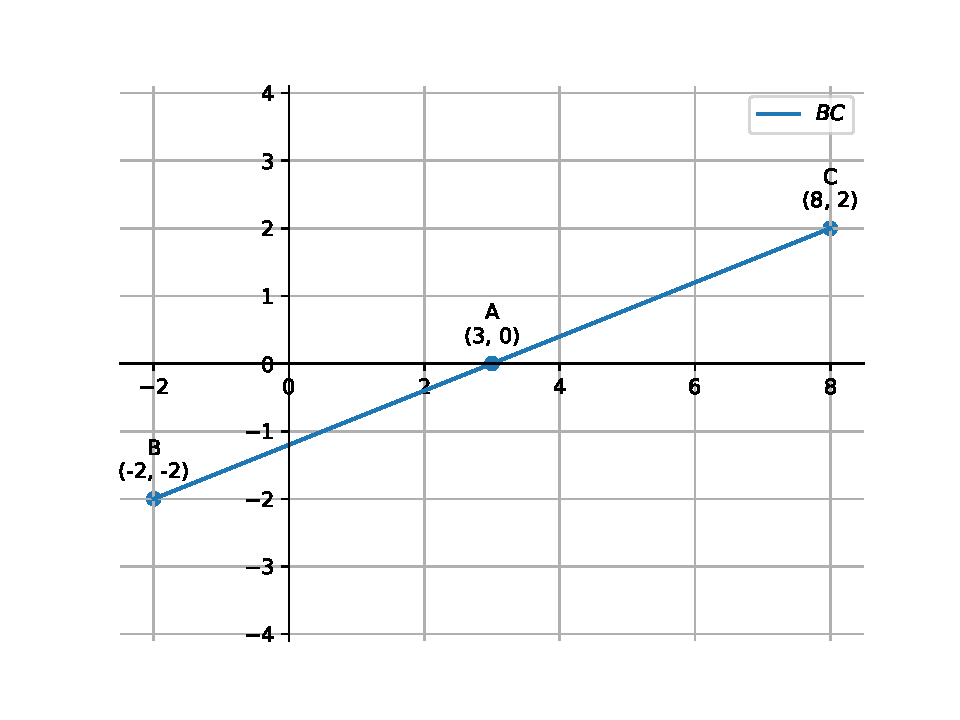
\includegraphics[width=0.75\columnwidth]{chapters/11/10/2/20/figs/fig.pdf}
		\caption{}
		\label{fig:11/10/2/20}
  	\end{figure}

\item Find the equation of the line  parallel to the line 3x-4y+2=0 and passing through the point (-2,3).
\label{chapters/11/10/3/7}
%\iffalse
% #######################################
% ########### FILL THESE IN #############
% #######################################
\def\mytitle{MATRICES}
\def\mykeywords{}
\def\myauthor{GOWTHAMI MANDAVA}
\def\contact{gowthamimandava999@gmail.com}
\def\mymodule{ Future Wireless Communication(FWC22012)}
% #######################################
% #### YOU DON'T NEED TO TOUCH BELOW ####
% #######################################
\newcommand{\myvec}[1]{\ensuremath{\begin{pmatrix}#1\end{pmatrix}}}
\let\vec\mathbf
\providecommand{\pr}[1]{\ensuremath{\Pr\left(#1\right)}}
\providecommand{\qfunc}[1]{\ensuremath{Q\left(#1\right)}}
\providecommand{\sbrak}[1]{\ensuremath{{}\left[#1\right]}}
\providecommand{\lsbrak}[1]{\ensuremath{{}\left[#1\right.}}
\providecommand{\rsbrak}[1]{\ensuremath{{}\left.#1\right]}}
\providecommand{\brak}[1]{\ensuremath{\left(#1\right)}}
\providecommand{\lbrak}[1]{\ensuremath{\left(#1\right.}}
\providecommand{\rbrak}[1]{\ensuremath{\left.#1\right)}}
\providecommand{\cbrak}[1]{\ensuremath{\left\{#1\right\}}}
\providecommand{\lcbrak}[1]{\ensuremath{\left\{#1\right.}}
\providecommand{\rcbrak}[1]{\ensuremath{\left.#1\right\}}}
\documentclass[10pt, a4paper]{article}
\usepackage[a4paper,outer=1.5cm,inner=1.5cm,top=1.75cm,bottom=1.5cm]{geometry}
\twocolumn
\usepackage{circuitikz}
\usepackage{amsmath,bm}
\usepackage{amsthm}
\usepackage{mathtools}
\usepackage{amsfonts}
\usepackage{amssymb}
\usepackage{graphicx}
\graphicspath{{./images/}}
%colour our links, remove weird boxes
\usepackage[colorlinks,linkcolor={black},citecolor={blue!80!black},urlcolor={blue!80!black}]{hyperref}
%Stop indentation on new paragraphs
\usepackage[parfill]{parskip}
%% Arial-like font
\usepackage{lmodern}
\renewcommand*\familydefault{\sfdefault}
%Napier logo top right
\usepackage{watermark}
%Lorem Ipusm dolor please don't leave any in you final report ;)
\usepackage{karnaugh-map} 
\usepackage{tabularx}
\usepackage{lipsum}
\usepackage{xcolor}
\usepackage{listings}
%give us the Capital H that we all know and love
\usepackage{float}
%tone down the line spacing after section titles
\usepackage{titlesec}
%Cool maths printing
\usepackage{amsmath}
%PseudoCode
\usepackage{algorithm2e}

\titlespacing{\subsection}{0pt}{\parskip}{-3pt}
\titlespacing{\subsubsection}{0pt}{\parskip}{-\parskip}
\titlespacing{\paragraph}{0pt}{\parskip}{\parskip}
\newcommand{\figuremacro}[5]{
    \begin{figure}[#1]
        \centering
        \includegraphics[width=#5\columnwidth]{#2}
        \caption[#3]{\textbf{#3}#4}
        \label{fig:#2}
    \end{figure}
}


 \lstset{
frame=single, 
breaklines=true,
columns=fullflexible
}

\thiswatermark{\centering \put(1,-110){\includegraphics[scale=0.05]{IIT_logo.jpg}} }
\title{\mytitle}
\author{\myauthor\hspace{1em}\\\contact\\IITH\hspace{0.5em}-\hspace{0.5em}\mymodule}
\date{}
\hypersetup{pdfauthor=\myauthor,pdftitle=\mytitle,pdfkeywords=\mykeywords}
\sloppy
% #######################################
% ########### START FROM HERE ###########
% #######################################
\begin{document}
 \maketitle
 \tableofcontents
 
    
 

 
    
    
    
 
 \Large\section{Problem}
 \fi
\\
\solution 
\iffalse
 \section{Solution}
 \begin{center}
 Given equation is 3x-4y+2=0
\\the parallel line passing through point(-2,3)
\begin{align}
\textbf{n}^{\top}(\textbf{x}-\textbf{p})=0 
\end{align}
\label{tab:truthtable}
    \setlength{\arrayrulewidth}{0.2mm}
\setlength{\tabcolsep}{5pt}
\renewcommand{\arraystretch}{1.25}
    \begin{tabular}{|c|c|}
    \hline % <-- Alignments: 1st column left, 2nd middle and 3rd right, with vertical lines in between
      \large\textbf{Symbol} & \large\textbf{Co-ordinates} \\
      \hline
       \large \textbf{n} & $\ \begin{pmatrix} 3\\ -4 \end{pmatrix}$  \\
       \hline
       \large p & $\ \begin{pmatrix} -2\\ 3 \end{pmatrix}$ \\
       \hline
       	\large c & 2 \\
      \hline
   \end{tabular}
\\ by substituting we get
\fi
From the given information, 
\begin{align}
{\vec{n}}=\myvec{3\\-4} \\
\implies 
	\myvec{3&-4}\cbrak{\vec{x}-\myvec{-2\\3}}&=0
	\\
	&=-18 
\end{align}
which is the required equation of the line.
\iffalse
  therefore,the equation parallel to the given equation and passing through the point(-2,3) is 3x-4y+18=0
 \end{center}
 \section{Plot}
         \centering
        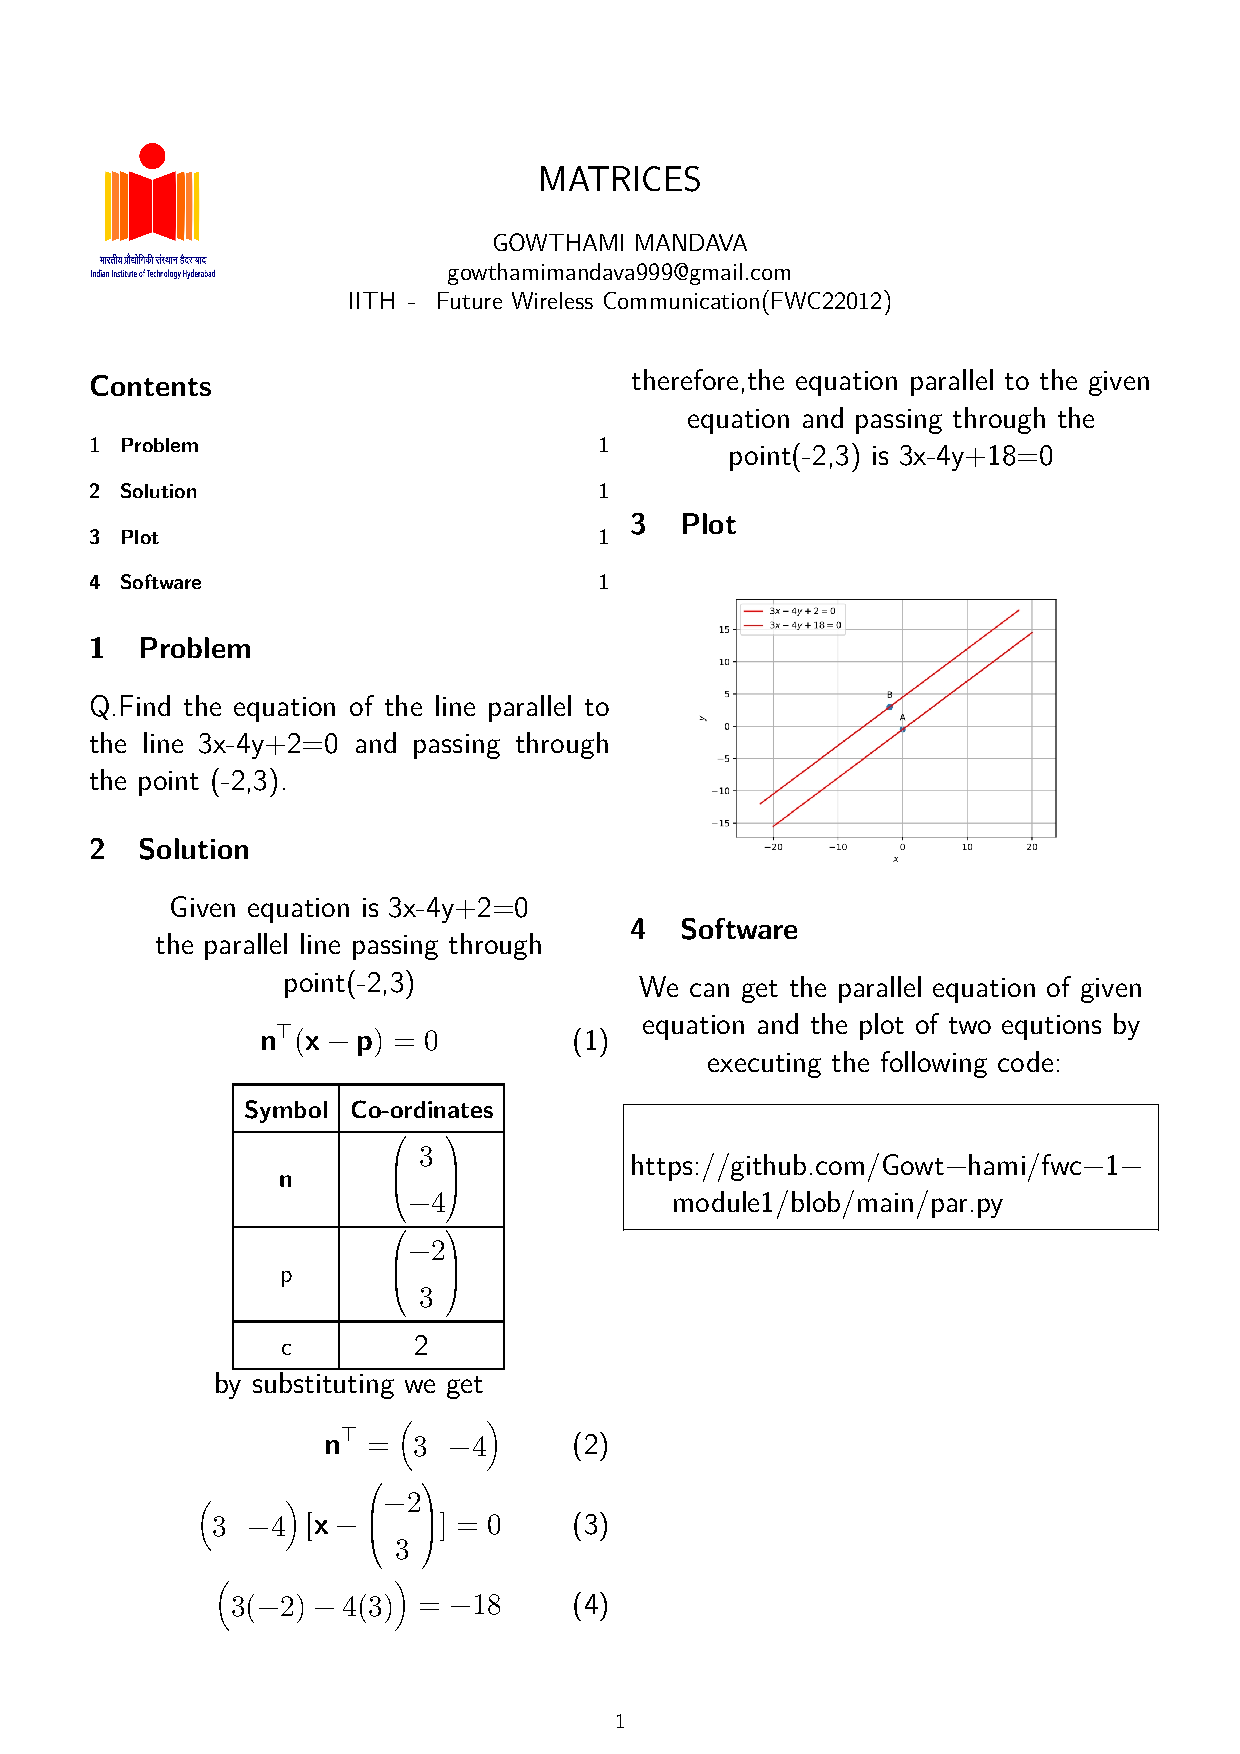
\includegraphics[scale=0.275]{mat.jpg}
  \section{Software}
  We can get the parallel equation of given equation and the plot of two equtions by executing the following code:
 \vspace{3mm} 
\begin{lstlisting}

https://github.com/Gowt-hami/fwc-1-module1/blob/main/par.py
\end{lstlisting}
\end{document}
\fi

\item Find the equation of line perpendicular to the line $x-7y+5=0$ and having $x$ intercept $3$\\
\label{chapters/11/10/3/8}
\solution
%The desired equation is
		\begin{align}
			\myvec{7 & 1}\brak{\vec{x}-\myvec{3\\0}} &=0\\
		\implies 	\myvec{7 & 1}\vec{x} &= 21
		\end{align}
		See 
\figref{fig:chapters/11/10/3/8/Fig1}.
		\begin{figure}[!h]
\begin{center}
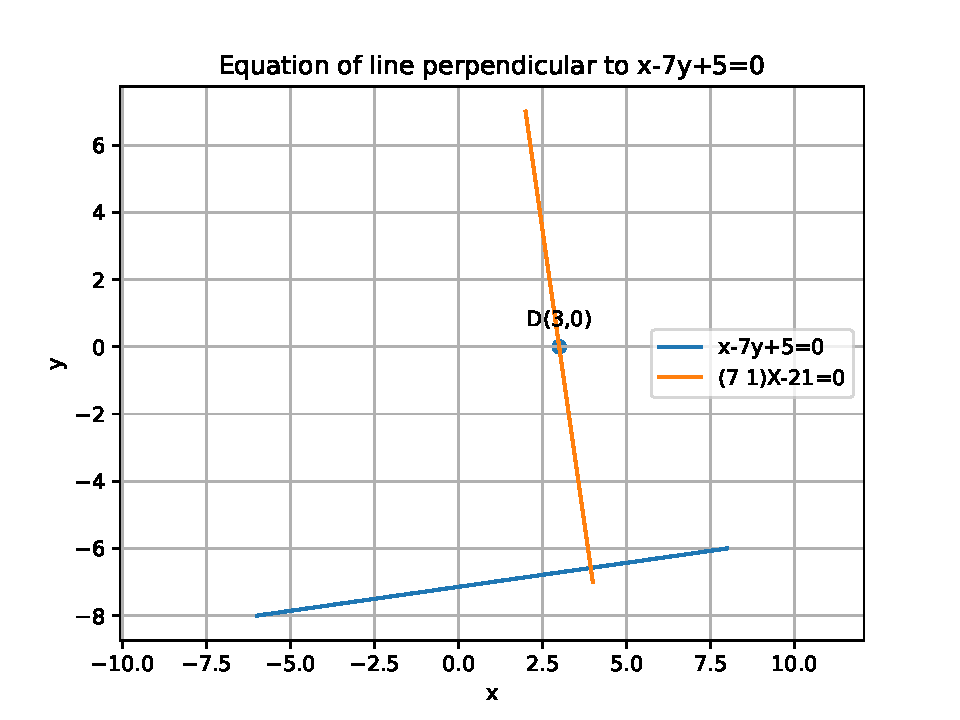
\includegraphics[width=\columnwidth]{chapters/11/10/3/8/figs/fig.pdf}
\end{center}
\caption{}
\label{fig:chapters/11/10/3/8/Fig1}
\end{figure}

\item Prove that the line through the point$(x_1,y_1)$ and parallel to the line A$x$+B$y$+C=0 is A$(x-x_1)$+B$(y-y_1)$=0.
\label{chapters/11/10/3/11}
\\
\solution
%\iffalse
\documentclass[10pt]{article}
\usepackage{graphicx}
\usepackage[none]{hyphenat}
\usepackage{graphicx}
\usepackage{listings}
\usepackage[english]{babel}
\usepackage{siunitx}
\usepackage{graphicx}
\usepackage{caption} 
\usepackage{booktabs}
\usepackage{array}
\usepackage{amssymb} % for \because
\usepackage{amsmath}   % for having text in math mode
\usepackage{extarrows} % for Row operations arrows
\usepackage{listings}
\usepackage[utf8]{inputenc}
\lstset{
  frame=single,
  breaklines=true
}
\usepackage{hyperref}
  
%Following 2 lines were added to remove the blank page at the beginning
\usepackage{atbegshi}% http://ctan.org/pkg/atbegshi
\AtBeginDocument{\AtBeginShipoutNext{\AtBeginShipoutDiscard}}


%New macro definitions
\newcommand{\mydet}[1]{\ensuremath{\begin{vmatrix}#1\end{vmatrix}}}
\providecommand{\brak}[1]{\ensuremath{\left(#1\right)}}
\newcommand{\solution}{\noindent \textbf{Solution: }}
\newcommand{\myvec}[1]{\ensuremath{\begin{pmatrix}#1\end{pmatrix}}}
\providecommand{\norm}[1]{\left\lVert#1\right\rVert}
\providecommand{\abs}[1]{\left\vert#1\right\vert}
\let\vec\mathbf{}
\begin{document}

\begin{center}
\title{\textbf{STRAIGHT LINES}}
\date{\vspace{-5ex}} %Not to print date automatically
\maketitle
\end{center}

\section{11$^{th}$ Maths - Chapter 10}
This is Problem 11 from Exercise-10.3
\begin{enumerate}
\item Prove that the line through the point$(x_1,y_1)$ and parallel to the line A$x$+B$y$+C=0 is A$(x-x_1)$+B$(y-y_1)$=0.

\solution
Given 
\fi
The given line parameters are
\begin{align}
\vec{n}=\myvec{A\\B}, \, c = C
\end{align}
Let 
\begin{align}
\vec{P}=\myvec{x_1\\y_1}\\
\end{align}
Then the equation of the desired line is
\begin{align}
	\vec{n}^\top\brak{\vec{x}-\vec{P}}&=0\\
	\implies A(x-x_1)+B(y-y_1)&=0
\end{align}

	\item Find the equation of the line passing through the point $\brak{1,2,-4}$ and perpendicular to the two lines
\begin{align}
	\frac{x-8}{3}=\frac{y+19}{-16}=\frac{z-10}{7} \text{ and }\\ \frac{x-15}{3}=\frac{y-29}{8}=\frac{z-5}{-5} 
\end{align}
    \solution
		%The direction vector of the desired line 
is given by 
\begin{align*}
	\myvec{3 & -16 & 7\\3 & 8 & -5}\vec{m} = 0
	\xleftrightarrow[]{R_2\leftarrow R_2-R_1}
 	\myvec{3 & -16 & 7\\0 & 24 & -12}
	\\
	\xleftrightarrow[]{R_1\leftarrow R_1+\frac{2}{3}R_2}
	\myvec{3 & 0 & -1\\0 & 24 & -12}
	\xleftrightarrow[]{R_2\leftarrow R_2/12}
	\myvec{3 & 0 & -1\\0 & 2 & -1}
\end{align*}
yielding
\begin{align}
	\vec{m} = \myvec{2\\3\\6}
\end{align}
Hence the vector equation of the line passing through $\brak{1,2,-4}$ is,
\begin{align}
	\vec{x} = \myvec{1\\2\\-4} + \kappa \myvec{2\\3\\6}
\end{align}



	\item  Find the vector equation of the line passing through $\myvec{1\\2\\3}$ and parallel to the planes $\myvec{1\\-1\\2}^{\top}\vec{x} = 5$ and $\myvec{3\\1\\1}^{\top}\vec{x} = 6$.  
    \solution
		%The direction vector of the line  is given by 
\begin{align*}
 \myvec{1&-1&2 \\ 3&1&1}\vec{m} = 0
 \xleftrightarrow[]{R_2\rightarrow -\frac{3}{4}{R_1} + \frac{1}{4}{R_2}} \myvec{1&-1&2 \\ 0&1&-\frac{5}{4}}\\
   \myvec{1&-1&2 \\ 0&1&-\frac{5}{4}} \xleftrightarrow[]{R_1\rightarrow {R_1} + {R_2}} \myvec{1&0&\frac{3}{4} \\ 0&1&-\frac{5}{4}}
   \\
 \implies \vec{m} =\myvec{-3\\5\\4}
\end{align*}
$\therefore$ the equation of the line is
\begin{align}
    \vec{x} = \myvec{1\\2\\3} + \lambda\myvec{-3\\5\\4} 
\end{align}


	\item
		%Using the scalar product
\begin{align}
  \cos{60\degree}=
\frac{1}{2}=\frac{\myvec{
        1&2
    }\myvec{
        1\\m
    }}{\sqrt{5}\sqrt{m^2+1}}\\
\implies 11m^2+16m-1=0\\
   or, m=\frac{-8\pm5\sqrt{3}}{11}    
\end{align}
So, the desired equation of the line is
\begin{align}
\myvec{
    \frac{-8\pm5\sqrt{3}}{11}&-1
}\vec{x} 
	&=
\myvec{
    \frac{-8\pm5\sqrt{3}}{11}&-1
}
\myvec{
    2\\3}
    \\
	&=\frac{-49\pm16\sqrt{3}}{11}
\end{align}
See 
    \figref{fig:11.10.3.12}.
\begin{figure}[!ht]
    \centering
    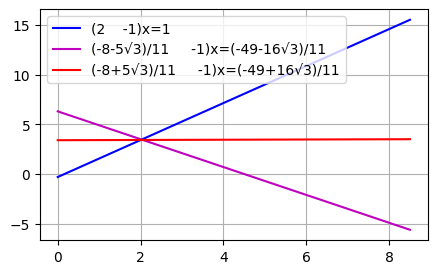
\includegraphics[width=\columnwidth]{chapters/11/10/3/12/fig/asgnt1.png}
    \caption{}
    \label{fig:11.10.3.12}
\end{figure}


\label{chapters/11/10/3/12}
\item
%Performing row operations
on the matrix
\begin{align*}  
\myvec{
    3 &1&-2 \\
     p&2&-3\\
     2&-1&-3
}
\xrightarrow[R_3=3R_3-2R_1]{R_2=3R_2-pR_1}&\myvec{
    3&1&-2\\
     $0$&6-p&-9+2p\\
     0&-5&-5}\\
 \xrightarrow{R_3=R_3(6-p)+5R_2}&\myvec{
    3&1&-2\\
     0&6-p&-9+2p\\
     0&0&-75+15p}
     \\
  \implies 
    p=5
\end{align*}
Substituting this value in the above, we obtain
\begin{align}
\myvec{
    3&1&-2\\
     0&1&1\\
     0&0&0}
\end{align}
yielding
\begin{align}
	\vec{x} = \myvec{-1 \\ 1}
\end{align}
as the point of intersection.
    See \figref{fig:11.10.4.9}.
\begin{figure}[H]
    \centering
    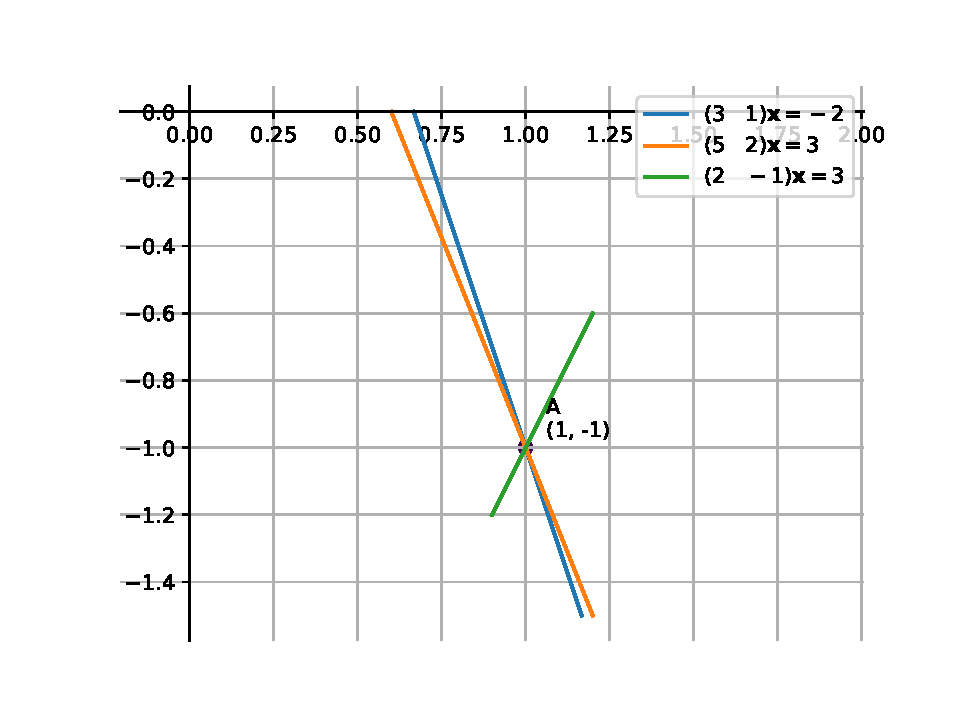
\includegraphics[width=0.75\columnwidth]{chapters/11/10/4/9/figs/fig.pdf}
    \caption{}
    \label{fig:11.10.4.9}
\end{figure}


%\label{11.10.4.9}
\item
	%Show that the line through the points \brak{4,7,8},\brak{2,3,4} is parallel to the line through the points\brak{-1,-2,1},\brak{1,2,5}.

\textbf{Solution :}
For line passing through \brak{4,7,8},\brak{2,3,4},the direction vector,\begin{align}
    \vec{m_1}&=\myvec{-2\\-4\\-4}
\end{align}
For line passing through \brak{-1,-2,1},\brak{1,2,5},the direction vector,\begin{align}
    \vec{m_2}&=\myvec{2\\4\\4}
\end{align}
Therefore,the lines are parallel to each other.

	\label{12.11.2.3}
 
 \item The perpendicular from the origin to the line $y=mx+c$ meets it at the point $(-1,2)$. Find the values of m and c.
 \solution
 %From \probref{chapters/11/10/2/15},
\begin{align}
	\vec{n} = \myvec{-1\\2} \implies m = \frac{1}{2}
\end{align}
Also, from the given equation of the line and the given point, 
\begin{align}
	c = \myvec{-m & 1}\myvec{-1\\2} = 
\frac{5}{2}  
\end{align}
\iffalse
 See \figref{fig:pic}.
\begin{figure}[H]
 \centering
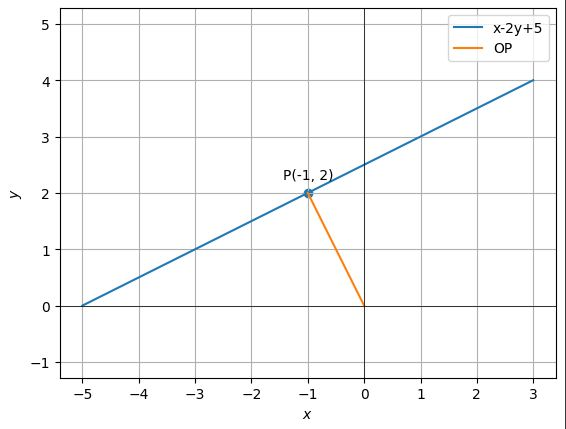
\includegraphics[width=0.75\columnwidth]{chapters/11/10/3/15/figs/graph.jpg}
 \caption{Graph}
 \label{fig:pic}
\end{figure}
\fi

 \label{11.10.3.15}
 \begin{figure}[!ht]
 \centering
 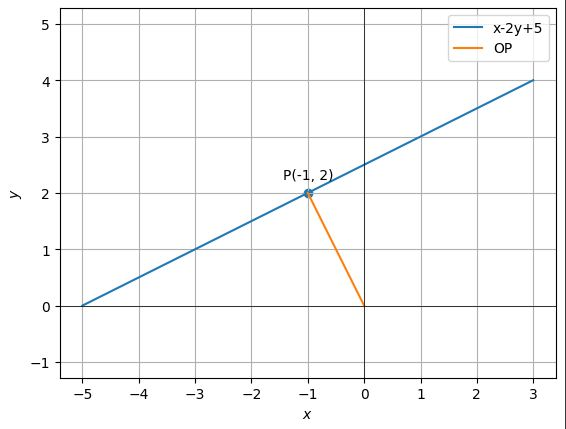
\includegraphics[width=\columnwidth]{chapters/11/10/3/15/figs/graph.jpg}
 \caption{Graph}
 \label{fig:pic}
 \end{figure}
\item Find the equation of the lines through the point (3, 2) which make an angle of 45\degree  with the line $x – 2y$ = 3.
\label{chapters/11/10/4/11}\\
\solution
%Following the approach in \probref{chapters/11/10/3/12},
\begin{align}
\cos45\degree =
\frac{1}{\sqrt{2}} = \frac{\myvec{2 & 1} \myvec{1\\m}}{\norm{\myvec{2\\1}}\norm{\myvec{1\\m}}}
\\
\implies 
 3m^2 - 8m -3 = 0
 \\
\text{or, }
m= - \frac{1}{3}, 3
\end{align} 
Thus, the desired equations are 
\begin{align}
	\myvec{1&3}\cbrak{\vec{x}-\myvec{3\\2}}&=0\\
 \implies 	\myvec{1 & 3}\vec{x} &= 9
\end{align}
and 
\begin{align}
	\myvec{3&-1}\cbrak{\vec{x}-\myvec{3\\2}}&=0\\
		\implies 	\myvec{3 & -1}\vec{x} &= 7
\end{align}
See
\figref{fig:chapters/11/10/4/11/figs/strline.jpg}.
\begin{figure}[H]
\centering
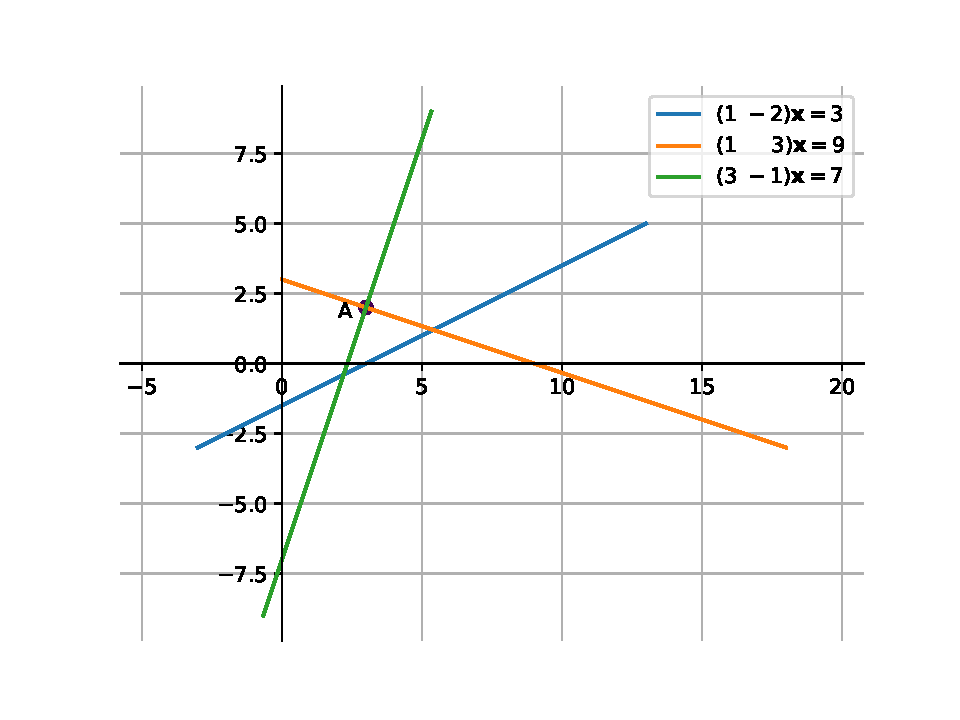
\includegraphics[width=0.75\columnwidth]{chapters/11/10/4/11/figs/fig.pdf}
\caption{}
\label{fig:chapters/11/10/4/11/figs/strline.jpg}
\end{figure}

\item Consider the following population and year graph, Find the slope of the line AB and using it, find what will be the population in the year 2010?
\\
\begin{figure}[!ht]
\centering
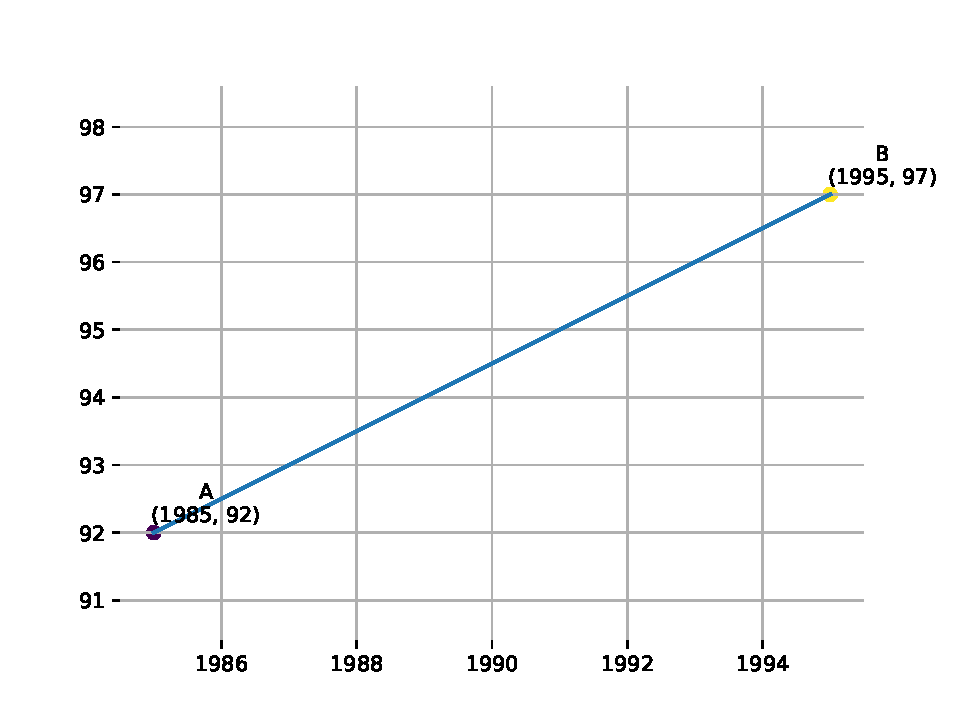
\includegraphics[width = \columnwidth]{chapters/11/10/1/14/figs/fig.png}
\caption{}
\label{fig:chapters/11/10/1/14/1}
\end{figure}
\solution
The direction vector of the line in \figref{fig:chapters/11/10/1/14/1} is
\begin{align}
\vec{m} = \vec{B} - \vec{A}
= \myvec{2 \\ 1}
\\
\implies \vec{n}
= \myvec{1 \\ -2}
\end{align}
 The equation of the line is then given by 
\begin{align}
\vec{n}^{\top} (\vec{x} -\vec{A}) &= 0 \\
\implies 
\myvec{1& -2} \vec{x} &= 1801
\\
\implies  \myvec{1&-2} \myvec{2010\\y} &= 1801 \\
\implies y &= \frac{209}{2}
\end{align}





 
\end{enumerate}
